\section{Effect of various hill shapes}
The velocity of waves on water is determined by the water depth. The q(x,y) function in our wave equation is
\begin{equation}
 q(x,y) = gH(x,y)
\end{equation}
where $H(x,y)$ is the water depth when the surface is flat.
We looked at three different sea bottoms; a beach shaped bottom, a bottom with an undersea mountain (gauss-form) and a box shape similar to the plug wave.

\begin{figure}[H]
\subfigure[The beach]{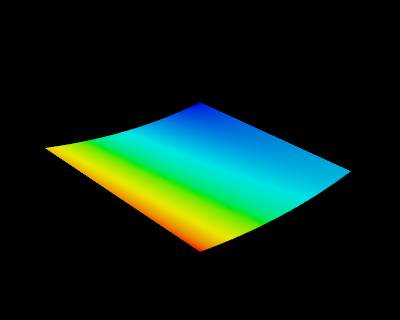
\includegraphics[width=0.4\textwidth]{beach.png}}
\subfigure[The mountain]{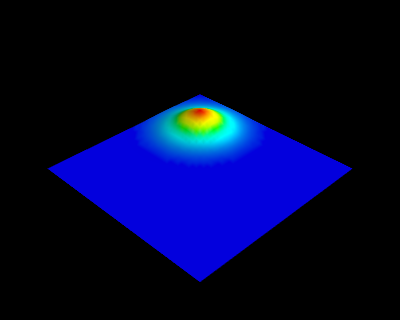
\includegraphics[width=0.4\textwidth]{mountain.png}}
\subfigure[The box]{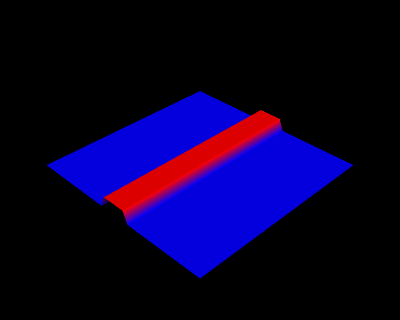
\includegraphics[width=0.4\textwidth]{box.png}}
\caption{The different sea bottoms}
\label{bottoms}

 \end{figure}

 Figure (\ref{bottoms}) show the three different sea bottoms we tested for. 
 
 \subsection{The beach}
 We used a gauss for out initial condition, and figure (\ref{beach}) show the time evolution of the waves for the beach-shaped sea bottom. We see that there is some noise when the wave moves towards the corner in the back. This is a bit weird 
since the sea bottom actually is a quite smooth surface. The reason that noise chose to be only in that corner
is because this is where the depth of the water is smallest. We believe there is a bug in our program, so maybe we can blame the noise on that bug.
 \begin{figure}[H]
\subfigure[beach pic 0]{\includegraphics[width=0.4\textwidth]{movie_pic_beach/wtmp0000.png}}
\subfigure[beach pic 2]{\includegraphics[width=0.4\textwidth]{movie_pic_beach/wtmp0005.png}}
\subfigure[beach pic 2]{\includegraphics[width=0.4\textwidth]{movie_pic_beach/wtmp0010.png}}
\subfigure[beach pic 3]{\includegraphics[width=0.4\textwidth]{movie_pic_beach/wtmp0015.png}}
\subfigure[beach pic 4]{\includegraphics[width=0.4\textwidth]{movie_pic_beach/wtmp0020.png}}
\subfigure[beach pic 5]{\includegraphics[width=0.4\textwidth]{movie_pic_beach/wtmp0025.png}}
\subfigure[beach pic 6]{\includegraphics[width=0.4\textwidth]{movie_pic_beach/wtmp0030.png}}
\subfigure[beach pic 7]{\includegraphics[width=0.4\textwidth]{movie_pic_beach/wtmp0035.png}}
%\subfigure[beach pic 8]{\includegraphics[width=0.4\textwidth]{movie_pic_beach/wtmp0008.png}}
%\subfigure[beach pic 9]{\includegraphics[width=0.4\textwidth]{movie_pic_beach/wtmp0009.png}}
\caption{The waves on a beach}
\label{beach}

\end{figure}





\subsection{The mountain}
Again we start out with a gauss-wave, but this time the sea bottom has a mountain in the corner. Figure (\ref{mountain})
shows the time evolution of the gauss wave over this type of bottom.
On the latest
plots in the time evolution ((d) - (h)) we clearly see that there is a mountain disrupting the waves in the back corner.
The waves over the mountain is not smooth (there is noise there), as one might expect.

\begin{figure}[H]
\subfigure[mountain pic 0]{\includegraphics[width=0.4\textwidth]{movie_pic_mountain/wtmp0000.png}}
\subfigure[mountain pic 2]{\includegraphics[width=0.4\textwidth]{movie_pic_mountain/wtmp0005.png}}
\subfigure[mountain pic 2]{\includegraphics[width=0.4\textwidth]{movie_pic_mountain/wtmp0010.png}}
\subfigure[mountain pic 3]{\includegraphics[width=0.4\textwidth]{movie_pic_mountain/wtmp0015.png}}
\subfigure[mountain pic 4]{\includegraphics[width=0.4\textwidth]{movie_pic_mountain/wtmp0020.png}}
\subfigure[mountain pic 5]{\includegraphics[width=0.4\textwidth]{movie_pic_mountain/wtmp0025.png}}
\subfigure[mountain pic 6]{\includegraphics[width=0.4\textwidth]{movie_pic_mountain/wtmp0030.png}}
\subfigure[mountain pic 7]{\includegraphics[width=0.4\textwidth]{movie_pic_mountain/wtmp0035.png}}
%\subfigure[beach pic 8]{\includegraphics[width=0.4\textwidth]{movie_pic_beach/wtmp0008.png}}
%\subfigure[beach pic 9]{\includegraphics[width=0.4\textwidth]{movie_pic_beach/wtmp0009.png}}
\caption{The waves over a mountain}
\label{mountain}

\end{figure}


\subsection{The box}
The gauss wave is the initial condition again, but now the bottom has a box shape. Figure (\ref{box}) 
shows the time evolution of the gauss wave over this bottom.
The disruption of the wave does mach the shape of the box, and there does not seem to be much noise, even though
the velocity of the wave is abruptly changed when the wave crosses the box. The smooth gaussian mountain on the other
hand made quite a bit of noise and the smoothest shapes of all the bottoms, the beach
\begin{figure}[H]
\subfigure[box pic 0]{\includegraphics[width=0.4\textwidth]{movie_pic_box/wtmp0000.png}}
\subfigure[box pic 2]{\includegraphics[width=0.4\textwidth]{movie_pic_box/wtmp0005.png}}
\subfigure[box pic 2]{\includegraphics[width=0.4\textwidth]{movie_pic_box/wtmp0010.png}}
\subfigure[box pic 3]{\includegraphics[width=0.4\textwidth]{movie_pic_box/wtmp0015.png}}
\subfigure[box pic 4]{\includegraphics[width=0.4\textwidth]{movie_pic_box/wtmp0020.png}}
\subfigure[box pic 5]{\includegraphics[width=0.4\textwidth]{movie_pic_box/wtmp0025.png}}
\subfigure[box pic 6]{\includegraphics[width=0.4\textwidth]{movie_pic_box/wtmp0030.png}}
\subfigure[box pic 7]{\includegraphics[width=0.4\textwidth]{movie_pic_box/wtmp0035.png}}
%\subfigure[beach pic 8]{\includegraphics[width=0.4\textwidth]{movie_pic_beach/wtmp0008.png}}
%\subfigure[beach pic 9]{\includegraphics[width=0.4\textwidth]{movie_pic_beach/wtmp0009.png}}
\caption{The waves over a box}
\label{box}

\end{figure}




